\documentclass[11pt]{article}
\usepackage[margin=1in]{geometry}
\usepackage{graphicx}
\usepackage{amsmath,amssymb}
\usepackage{booktabs}
\usepackage{listings}
\usepackage{xcolor}
\usepackage[colorlinks=true,linkcolor=blue,citecolor=blue,urlcolor=blue]{hyperref}
\graphicspath{{figs/}}

\lstset{basicstyle=\ttfamily\small, breaklines=true, frame=single,
        showstringspaces=false,
        backgroundcolor=\color{gray!8}, columns=fullflexible,
        xleftmargin=2mm, framexleftmargin=2mm}

\newcommand{\vcut}{v_{\mathrm{cut}}}
\newcommand{\sobs}{\sigma_{\mathrm{obs}}}
\newcommand{\sborn}{\sigma_{\mathrm{Born}}}
\newcommand{\code}[1]{\texttt{#1}}

\title{\textbf{exclurad\_py: user manual}\\[2mm]
\large Exclusive meson electroproduction with exact radiative corrections}
\author{V.~Kubarovsky\\ \small Jefferson Lab}
\date{\today}

\begin{document}
\maketitle

\begin{abstract}
\code{exclurad\_py} generates exclusive meson electroproduction events
$ep\to e'\,h\,X$ for $\pi^0$, $\eta$, $\rho$, $\phi$ and $J/\psi$ with exact
first-order QED radiative corrections on the EXCLURAD framework, and with
pre-vertex external radiation in the target. This manual is what you need to
run it: how to get the code, what the directory tree means, every field of
the run card, how the radiative correction is extracted from a pair of runs,
and what to change to add a new structure-function model. It is deliberately
short; the physics, the validation and the evidence are in the companion
note.
\end{abstract}

\tableofcontents

\section{Getting the code}

The repository is \url{https://github.com/vkubarovsky/exclurad_py}. Production
runs must use a tagged commit, never a branch tip: the tag is written into
every output file and is how a sample is traced back to the code that made it.

\begin{lstlisting}[language=bash]
git clone -b feature/exclurad_py git@github.com:vkubarovsky/exclurad_py.git
cd exclurad_py
git checkout prod-pi0-v1          # a tag, not a branch
git describe --tags               # must echo the tag back
\end{lstlisting}

Requirements are only \code{python3} and \code{numpy}; \code{matplotlib} is
needed for the plotting tools, not for generation. Versions in use range from
python 3.9 with numpy 1.23 on the JLab farm to python 3.14 with numpy 2.4 on
macOS, and both give statistically identical samples; the cross-machine
comparison is in the companion note.

\paragraph{Deploying to a machine without GitHub access.}
\code{production/deploy.sh} copies the tree and writes
\code{exclurad\_py/DEPLOYED\_VERSION} beside the package, which the provenance
code reads when \code{.git} is absent. Use it only when a clone is impossible:
a real clone lets \code{git describe} verify the version \emph{on the machine},
while the file merely asserts it.

\section{Directory tree}

\begin{lstlisting}
exclurad_py/               the repository
  exclurad_py/             the python package (import root)
    core/                  kinematics, Born, rc_factor -- the physics
    models/                structure-function models, one class each
    generator/             sampling, tables, decay, LUND writer
    topology.py            which hadron is detected; sign conventions
    runcard.py             the run-card parser
  cards/                   run cards, one per channel
  production/              run scripts, validation and plotting tools
  validation/              reports and reference data
  doc/                     this manual and the note
\end{lstlisting}

Output is written \emph{outside} the repository, into a directory you name in
the run card. The recommended layout, produced by
\code{production/run\_prod\_v1.sh}:

\begin{lstlisting}
<data>/pi0_v1/
  README.md          box, code version, checks the version rests on
  card_rad.txt       the cards actually used
  card_born.txt
  part_runner.py     written by the run script; nothing lives outside
  cyc01/ cyc02/ ...  one directory per cycle
    pi0/<date>_<E>_<mode>_v1/lund/*.lund
    logs/
  STOP               create this file to stop the loop cleanly
\end{lstlisting}

Cycles are independent: each has its own seed, and samples from different
cycles and different machines add up. To stop a running production,
\code{touch STOP} and the loop finishes its cycle and exits. Do not kill the
processes.

\section{The run card}

Plain text, one value per line, \code{!} starts a comment. The \emph{order of
the lines is the format} --- there are no keywords. Blank and comment-only
lines are skipped. Fortran exponents (\code{1.0d-4}) are accepted.

\begin{center}
\small
\begin{tabular}{rlp{9.2cm}}
\toprule
\# & field & meaning \\
\midrule
1  & model      & \code{<channel>.<vintage>}, e.g.\ \code{pi0.vpk2021}. Not an
                  integer channel code: several vintages of the same channel
                  give visibly different RC, and the name goes into the output
                  header. \code{--models} lists them. \\
2  & ebeam      & beam energy, GeV \\
3  & nev        & events to write \\
4  & iborn      & 1 = Born only, 0 = full RC \\
5  & W2 range   & GeV$^2$ \\
6  & Q2 range   & GeV$^2$ \\
7  & t range    & GeV$^2$, both negative \\
8  & vcut       & $\vcut = M_X^2 - m_U^2$, GeV$^2$; 0 = generate to the
                  kinematic limit \\
9  & t\_nucl    & GeV$^2$, $\pi^0/\eta$ models only; ignored for vector mesons \\
10 & ihel       & $+1$, $-1$, or 0 = draw the helicity per event \\
11 & seed       & \\
12 & idecay     & 1 = decay the meson, 0 = leave it \\
13 & output root& \code{<channel>/<date>\_<E>\_<mode>\_v1/} is created under it \\
\midrule
\multicolumn{3}{l}{\emph{optional, may be omitted from the end}}\\
14 & y range    & $\nu/E$ \\
15 & xB range   & \\
16 & iacc       & acceptance preset: \code{none} or \code{jpsi} \\
17 & vmin       & soft/hard separator, GeV$^2$; 0 = choose automatically \\
18 & itarg      & 1 = pre-vertex external radiator in the target \\
19 & vz range   & cm, the target cell, e.g.\ \code{-7.5 -2.5} \\
\bottomrule
\end{tabular}
\end{center}

\paragraph{Two fields that are easy to confuse.}
\code{vcut} is \emph{physics}: the exclusivity cut of the analysis
($0.20\;\mathrm{GeV}^2$ for $\pi^0$ and $\eta$, $1.20$ for $J/\psi$).
\code{vmin} is \emph{arithmetic}: the internal soft/hard separator of the
Bardin--Shumeiko decomposition, conventionally $10^{-4}$. Nothing physical may
depend on \code{vmin}, and the note shows that nothing does.

\paragraph{\code{itarg} and the meaning of \code{vcut}.}
With the radiator on, \code{vcut} is applied in \emph{true} variables, at the
event's own reduced beam energy. An analysis cuts on the \emph{reconstructed}
missing mass, using the nominal beam energy, and about $0.8\,\%$ of the events
will fail that cut. This is correct and the sample is complete: external
energy loss can only raise the reconstructed inelasticity,
$v_{\rm rec}-v_{\rm true} = 2\,\Delta E\,(E_X-p_{X,z}) \ge 0$, so events leave
the window and never enter it.

\section{The mass of a vector meson}
\label{sec:bw}

For $\rho$, $\phi$ and $\omega$ the meson mass is \emph{not} a constant. It is
drawn per event from a Breit--Wigner --- with the running $p$-wave width for
$\rho$ --- and carried through the kinematics, the $t$ limits, the $W$
threshold, the Born cross section, the radiative correction and the decay.
Nothing in the card switches this on: it is on, because for $\rho$
($\Gamma=150$~MeV at $M=775$~MeV) a fixed mass is simply wrong, and for
$\phi$ the same machinery costs nothing. $J/\psi$, $\pi^0$ and $\eta$ are
narrow enough that the code treats them as $\delta$-functions, which is exact
at their widths.

Two consequences for the user of a sample. The written meson mass differs
event by event, so reconstruct it from the daughters rather than assuming the
PDG value. And the cross section is not the one at the pole: for $\rho$ over
the standard box it is $8\,\%$ lower, because the Breit--Wigner average of
$\sborn$ is not $\sborn$ at $M_0$.

\begin{figure}[htbp]
\centering
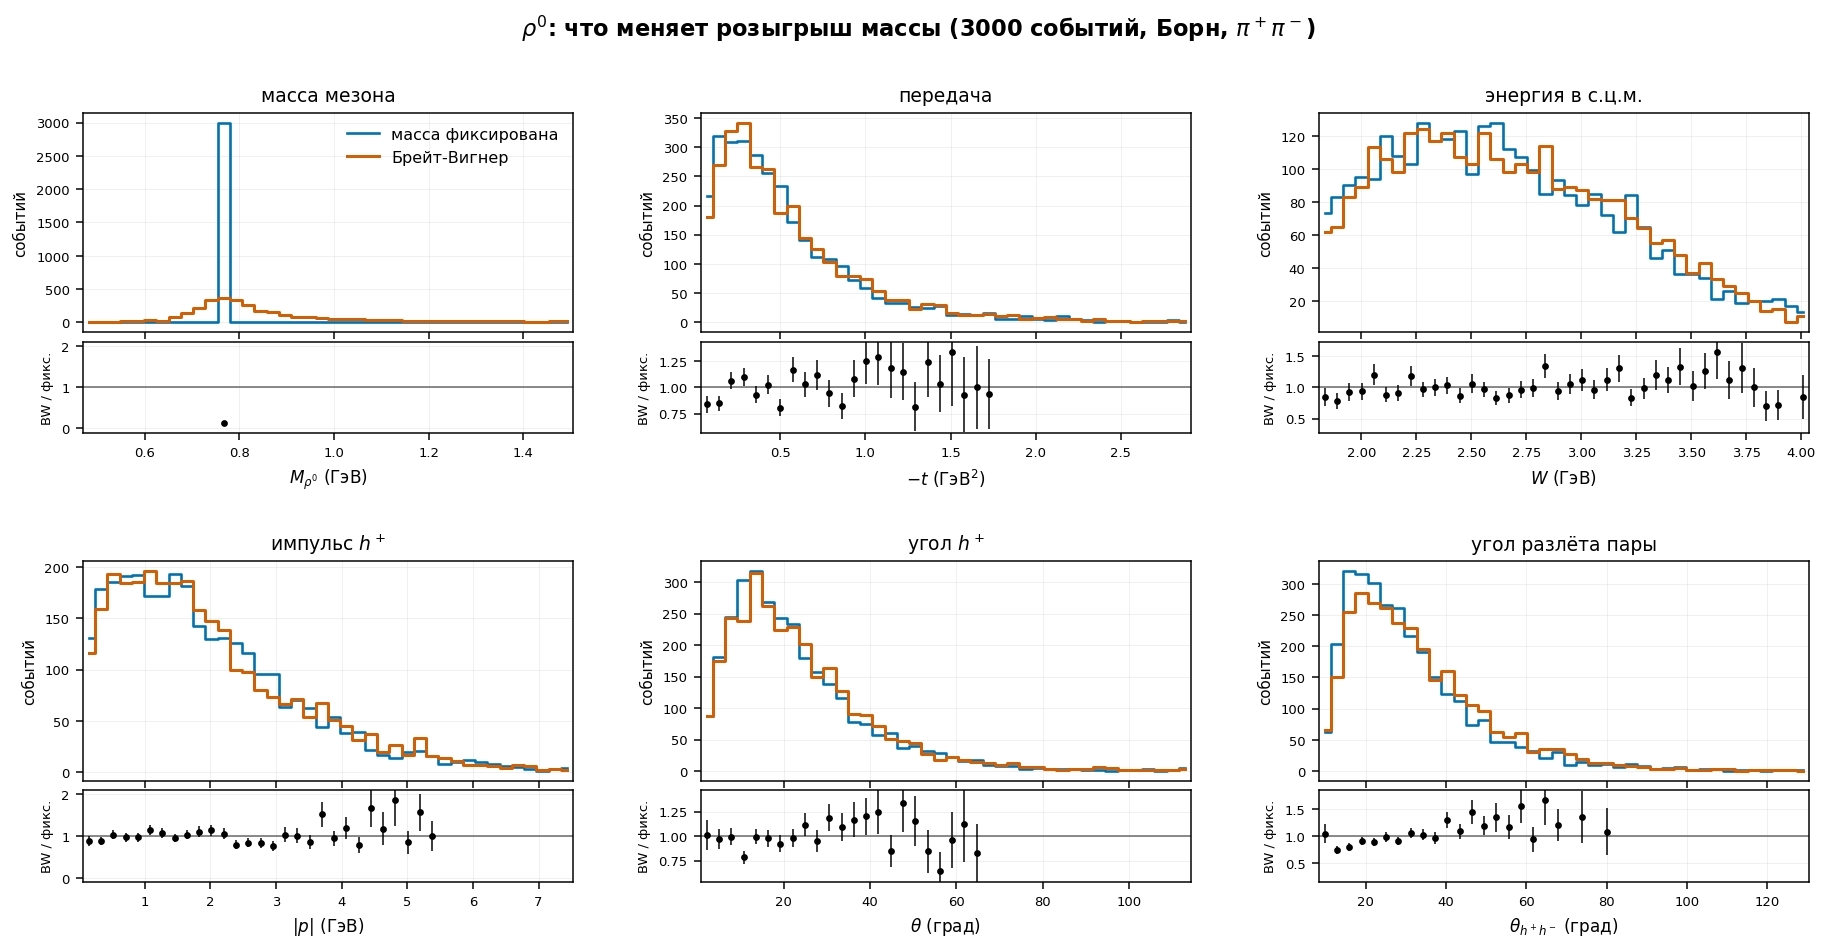
\includegraphics[width=\textwidth]{bw_look_rho.png}
\caption{$\rho$: mass fixed at the pole (blue) against the Breit--Wigner
draw (orange), same seed and same card. The peak is the obvious part; the
point is what the mass drags with it --- $|t|$, the $\pi^+$ momentum and
angle, the pair opening angle. These are the tracks the detector sees.}
\end{figure}

\paragraph{Turning it off.} \code{BW=0} in the environment restores the fixed
mass. It exists for validation --- with the draw off the generator reproduces
its pre-Breit--Wigner output byte for byte --- and for reproducing an old
sample. It is not a physics option for $\rho$ or $\phi$. Whether the draw was
active is recorded in the run's \code{report.bw\_channel}, so a sample can be
asked rather than assumed.

\section{Running}

One part of a run:

\begin{lstlisting}[language=bash]
export PYTHONPATH=$PWD
export TABLE_SERIAL=1 ETA_PROPOSAL_CAP=5 EXACT_ACCEPT=1 EXPO_TAIL=1
python3 -c "from exclurad_py.run import run; run('cards/rad_pi0.txt')"
\end{lstlisting}

\paragraph{Environment variables.} The card carries the physics; these carry
the numerics, and the four in the line above are what every production run
sets.

\begin{center}
\small
\begin{tabular}{lll p{7.0cm}}
\toprule
variable & default & production & meaning \\
\midrule
\code{EXACT\_ACCEPT}     & 0 & \textbf{1} & Second acceptance stage against
  the exact \code{rc\_factor} at the event's own kinematics, rather than
  against the interpolated table. This is what makes the sample carry the
  exact correction; it also forces the per-event photon path. \\
\code{EXPO\_TAIL}        & 0 & \textbf{1} & YFS exponentiation of the soft
  factor (scheme A). Also forces the per-event path. \\
\code{TABLE\_SERIAL}     & 0 & \textbf{1} & Build the $\eta$ table in one
  process. Slower, but the parallel build has hung in pool shutdown on
  python 3.14. \\
\code{ETA\_PROPOSAL\_CAP}& --- & \textbf{5} & Ceiling on the interpolated
  $\eta$ used as the sampling proposal. Caps efficiency loss from a table
  outlier; cannot bias the sample, because the second stage is exact. \\
\code{BW}                & 1 & 1 & Breit--Wigner mass draw, §\ref{sec:bw}.
  Set to 0 only to reproduce a pre-Breit--Wigner sample. \\
\code{MAJ\_SAFETY}       & 1.6 & --- & Margin on the majorant. Raise it if the
  \code{health:} line reports violations. \\
\code{MAJ\_SHAPE}        & --- & --- & Override the majorant grid. \\
\code{CARD}, \code{CARD\_PREFIX} & --- & --- & Which card the analysis tools
  read; see §\ref{sec:check}. \\
\bottomrule
\end{tabular}
\end{center}

For anything larger use \code{production/run\_prod\_v1.sh}, which splits the
work over cores, writes the README and the cards into the output directory,
and loops until a deadline:

\begin{lstlisting}[language=bash]
production/run_prod_v1.sh <code_dir> <out_dir> <seed_base> <ncores> <deadline_epoch> <label>
\end{lstlisting}

On a batch farm use \code{production/slurm\_submit.sh}, which submits the
table-building part first and the rest as an array depending on it. Building
the $\eta$ table once and letting the array read it from cache is not an
optimisation: launched together, the tasks race for the same file.

\section{Extracting the radiative correction}

Run the same card twice, changing only \code{iborn}, and the correction is the
ratio of the two samples bin by bin:
\begin{equation}
\delta(\mathrm{bin}) \;=\;
\frac{N_{\rm rad}(\mathrm{bin})/N_{\rm rad}}
     {N_{\rm born}(\mathrm{bin})/N_{\rm born}}
\;\times\;\frac{\sobs}{\sborn},
\qquad
\frac{\Delta\delta}{\delta}=\sqrt{\frac{1}{n_{\rm rad}}+\frac{1}{n_{\rm born}}}.
\end{equation}
Both samples come from the same generator, so the ratio tests the radiative
machinery and nothing else. Born events are about ten times cheaper, so make
the Born sample five times larger and its contribution to the error becomes
negligible.

\code{production/report\_run.py} does this for twelve variables at once:

\begin{lstlisting}[language=bash]
python3 production/report_run.py <run_dir> -c pi0
\end{lstlisting}

\begin{figure}[htbp]
\centering
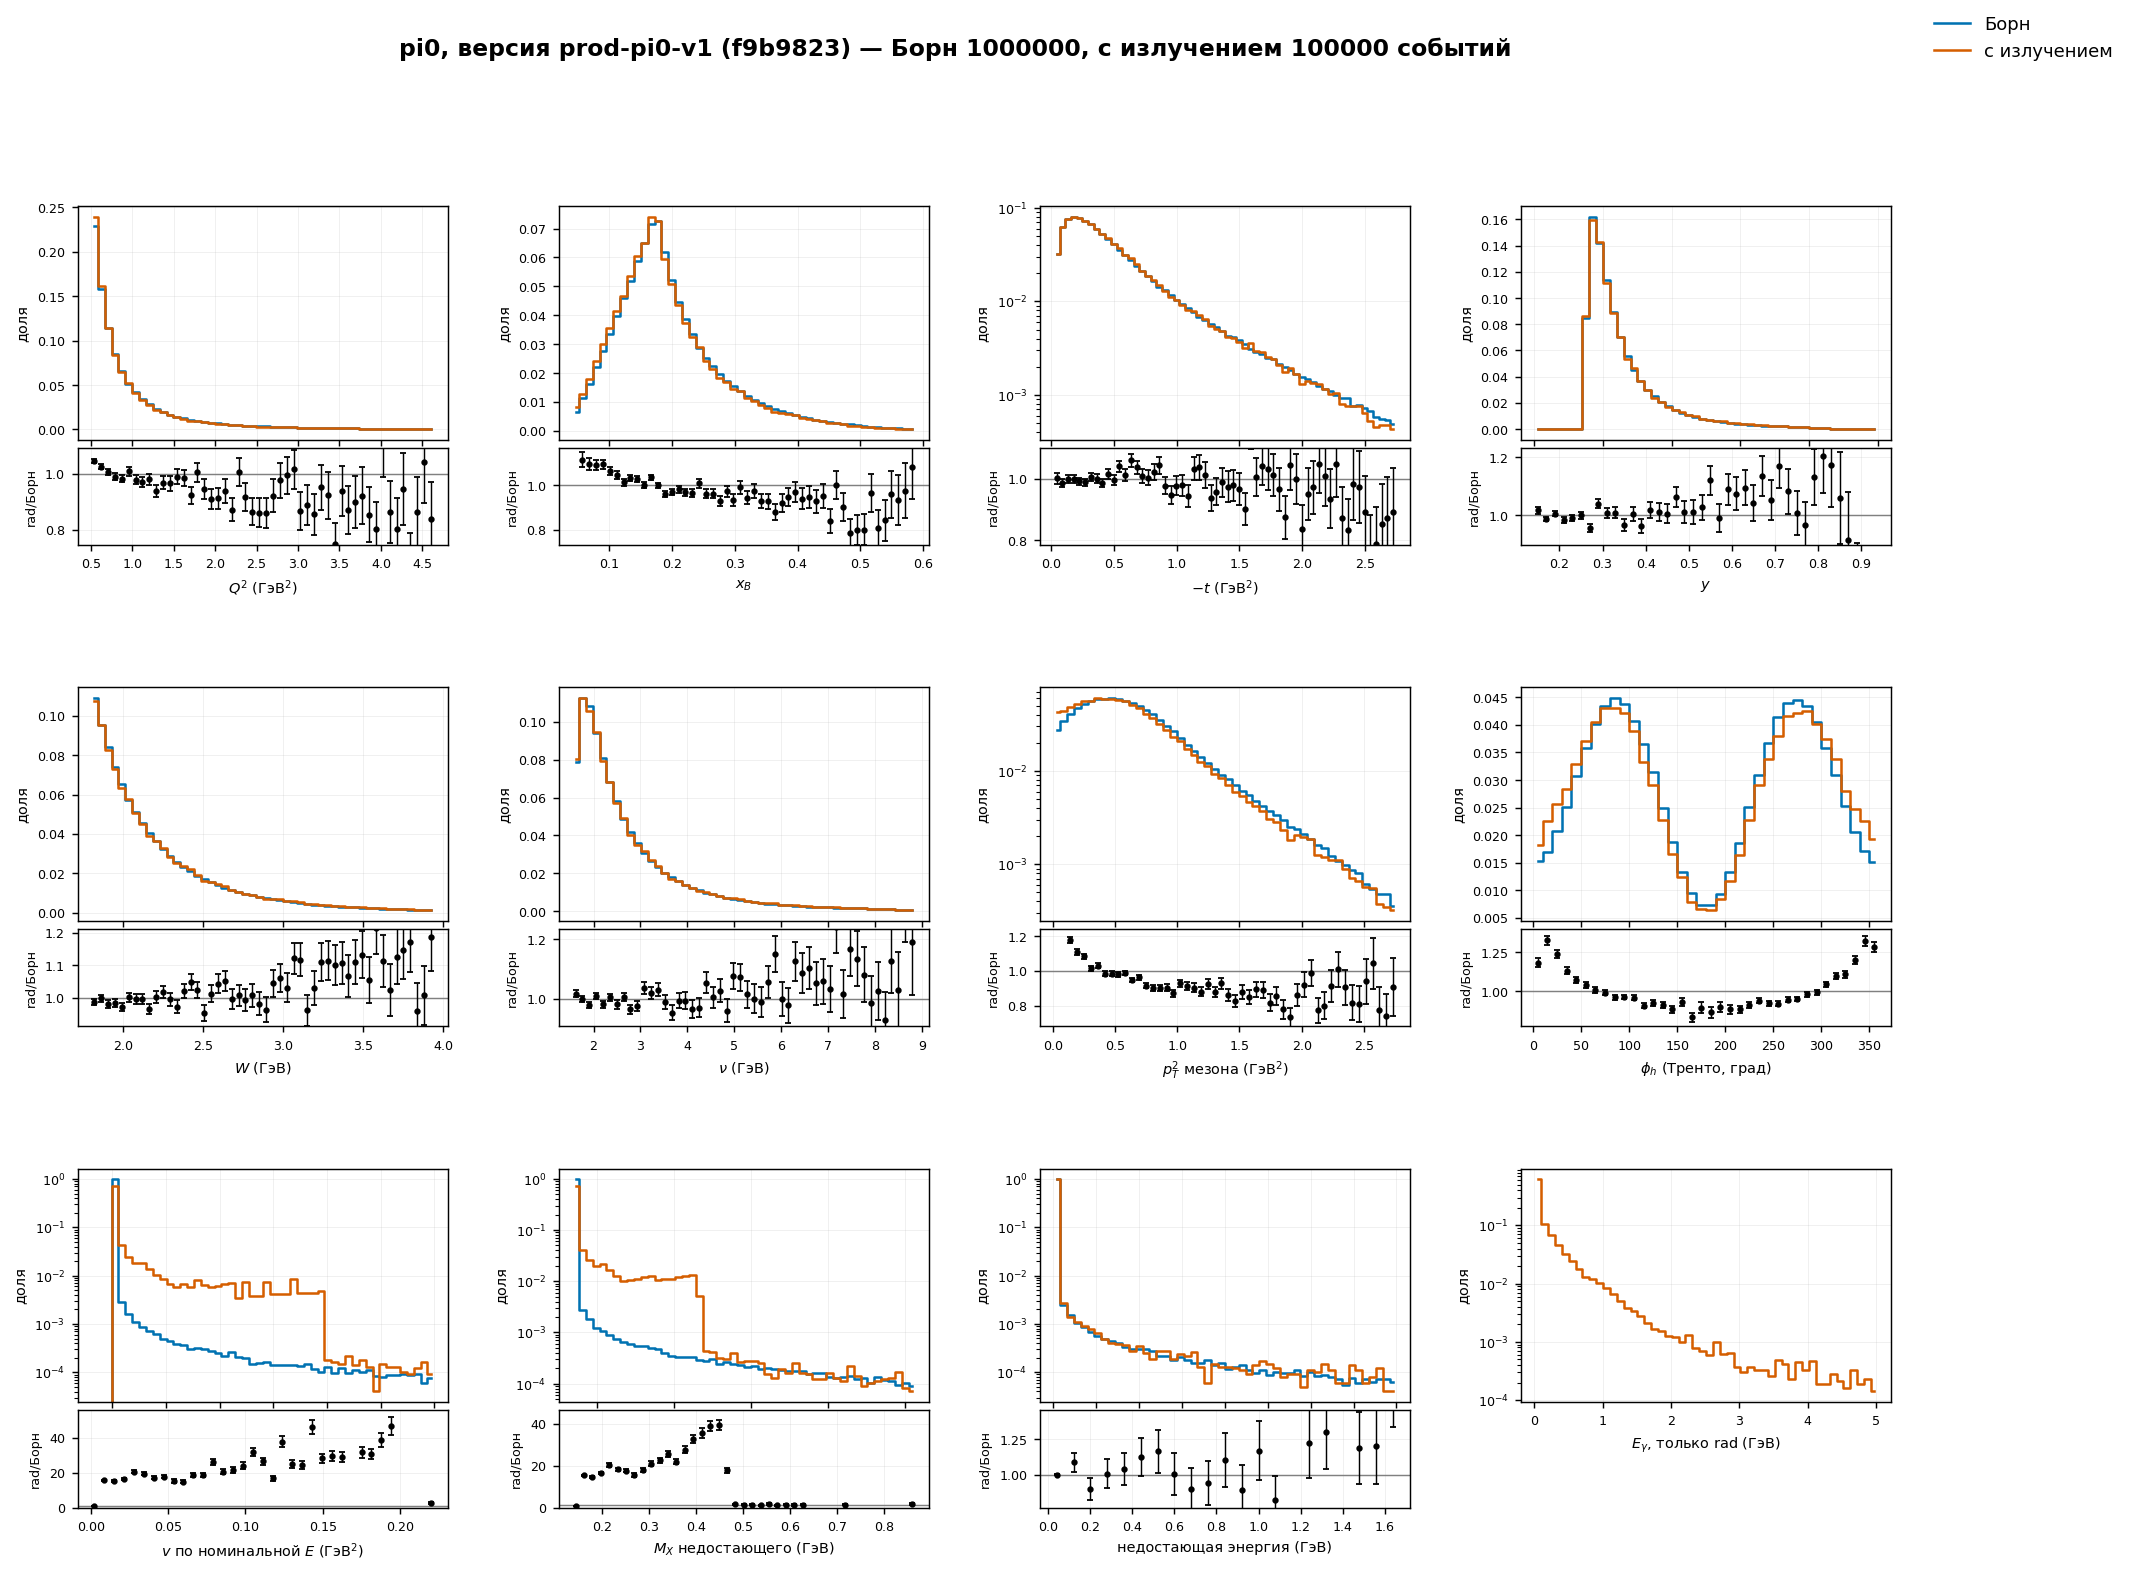
\includegraphics[width=\textwidth]{report_example.png}
\caption{Output of \code{report\_run.py}. Upper half of each cell: the Born and
radiative distributions, each normalised to unit area. Lower half: their ratio,
which \emph{is} the radiative correction as a function of that variable,
measured on the events with no quadrature involved. The strongest dependence is
on the azimuth, from $1.25$ to $0.85$.}
\label{fig:report}
\end{figure}

\section{Adding a structure-function model}

A model is one class in \code{exclurad\_py/models/}. It states its
provenance, its validity range and its topology, and implements one method
returning the five structure functions in nb/GeV$^2$:

\begin{lstlisting}[language=Python]
class MyModel(StructureFunctions):
    name       = "pi0.mine2027"
    channel    = "pi0"
    version    = "2027"
    provenance = "fit to <data>, table N of <note>"
    reference  = "arXiv:....."
    validity   = dict(W2=(3.2, 16.0), Q2=(0.5, 5.0), t=(-3.0, -0.001))
    topology   = baryon_detected(0.1349768, meson="pi0")

    def _sfs(self, W2, Q2, t):
        return dict(sT=..., sL=..., sTT=..., sLT=..., sLTp=...)
\end{lstlisting}

Register it in \code{models/\_\_init\_\_.py} and the name works in any card.

\paragraph{Four things to get right.}
\emph{Topology} decides which hadron is detected, and with it the sign of
$\sigma_{LT}$ and the azimuth offset; do not set those by hand. \emph{Units}
are nb/GeV$^2$ in the Hand convention. \emph{validity} is not bureaucracy: the
radiative tail evaluates the model at shifted kinematics, so a fit made on a
limited grid \emph{will} be called outside it, and the excursions are counted
and reported. And a moment known only as a \emph{fraction} of
$\sigma_U=\sigma_T+\varepsilon\sigma_L$ --- say
$\sigma_{LT'}/\sigma_U = 0.10$ --- is declared as
\code{SLTP\_OVER\_SU = 0.10} rather than written into \code{\_sfs}: the base
class then builds it from $\sigma_U$ at the event's own $\varepsilon$, which
needs the beam energy and stays correct when $\sigma_L$ stops being zero.

\section{Checking a sample}
\label{sec:check}

\begin{center}
\small
\begin{tabular}{lp{10.2cm}}
\toprule
tool & what it answers \\
\midrule
\code{check\_lund.py}       & Is the output internally consistent? Four-momentum,
                              mass shells, decay closure, charge, header. \\
\code{report\_run.py}       & What does the correction look like in twelve
                              variables? \\
\code{rc\_proof\_phi.py}    & Does the event density reproduce the exact
                              calculation? Events against quadrature in $\phi$. \\
\code{delta\_profiles.py}   & The same in $Q^2$, $W$, $|t|$, $\phi$. \\
\code{soft\_limit.py}       & Do radiative events with $v\to0$ become Born? \\
\code{compare\_machines.py} & Do two machines give the same sample? \\
\code{bw\_look.py}          & What does the Breit--Wigner draw change? Two
                              samples overlaid, mass fixed against mass drawn. \\
\code{bw\_closure.py}       & Is the mass spectrum the one it should be?
                              Events against BW$/N(W^2)\times\int\sborn$. \\
\code{estimate\_rate.py}    & How long will this card take, before starting? \\
\bottomrule
\end{tabular}
\end{center}

Two habits worth keeping. Point the tools at the right card: they read
\code{cards/rad\_<ch>.txt} unless \code{CARD} or \code{CARD\_PREFIX} says
otherwise, and a sample measured against the wrong card fails silently rather
than loudly. And read the \code{health:} line of every run --- it reports
majorant violations, which bias an unweighted sample and cannot be repaired
afterwards.

\end{document}
